\documentclass[paper=letter, fontsize=12pt]{article}
\usepackage{geometry}
\geometry{margin=1in}
\usepackage{graphicx}
\graphicspath{{/}}
\usepackage{amssymb}

%opening
\title{Compsci 571 HW1}
\author{Yilin Gao (yg95)}

\begin{document}

\maketitle

\section{Perceptron Algorithm and Convergence Analysis}

\begin{enumerate}
\item Perceptrons can be used to represent many Boolean functions $f: \{0, 1\} \rightarrow \{0, 1\}$ in n-dimensional space.
\begin{enumerate}
	\item Provide a two-input Boolean function $y = f(x_1, x_2)$, where $y, x_1, x_2 \in \{0, 1\}$, that can be represented by a single perceptron. Plot the points $(x_1, x_2)$ that represent all possible pair values (e.g. (0, 0), (0, 1), (1, 0), (1, 1)) and provide a separating hyperplane on the same figure.
	
	\textbf{Answer:}
	
	The function $y$ can be:
	
	\begin{tabular} {|c|c|c|}
		\hline
		$y$ & $x_1$ & $x_2$	\\ \hline
		0 & 0 & 0 \\ \hline
		1 & 0 & 1 \\ \hline
		1 & 1 & 0 \\ \hline
		1 & 1 & 1 \\ \hline
	\end{tabular} \\

	One possible separating hyperplane can be: $f(x_1, x_2) = x_1 + x_2 - 0.5$. 
	
	Plot: 
	
	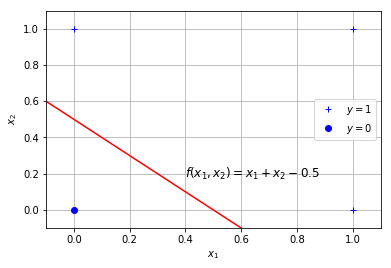
\includegraphics[scale=0.5]{1a.png}
	
	\item Provide a two-point Boolean function $y = f(x_1, x_2)$ that cannot be represented by a single perceptron. Briefly explain why.
	
	\textbf{Answer:}
	
	The function $y$ can be:
	
	\begin{tabular} {|c|c|c|}
		\hline
		$y$ & $x_1$ & $x_2$	\\ \hline
		0 & 0 & 0 \\ \hline
		1 & 0 & 1 \\ \hline
		1 & 1 & 0 \\ \hline
		0 & 1 & 1 \\ \hline
	\end{tabular} \\

	This is because these data are not linearly separable (in this case, fully separated by a line). According to the properties of Perceptron algorithm, if the training data are not linearly separable, the algorithm will fail.
	
	\item Provide a three-input Boolean function $y = f(x_1, x_2, x_3)$, where $y, x_1, x_2, x_3 \in \{0, 1\}$, that can be represented by a single perceptron. Plot the points $(x_1, x_2, x_3)$ that represent all possible pair values and provide a separating hyperplane on the same figure.
	
	\textbf{Answer:}
	
	The function $y$ can be:
	
	\begin{tabular} {|c|c|c|c|}
		\hline
		$y$ & $x_1$ & $x_2$	& $x_3$\\ \hline
		0 & 0 & 0 & 0\\ \hline
		0 & 1 & 0 & 0 \\ \hline
		0 & 0 & 0 & 1 \\ \hline
		0 & 1 & 0 & 1 \\ \hline
		1 & 0 & 1 & 0\\ \hline
		1 & 1 & 1 & 0 \\ \hline
		1 & 0 & 1 & 1 \\ \hline
		1 & 1 & 1 & 1 \\ \hline
	\end{tabular} \\

	One possible separating hyperplane can be: $f(x_1, x_2, x_3) = x_2 - 0.5$
	
	Plot:
	
	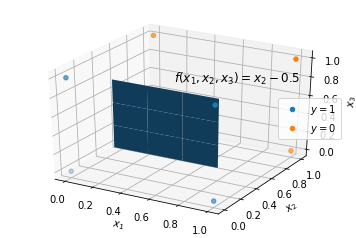
\includegraphics[scale=0.6]{1c.png}
	
\end{enumerate}

\item For a response variable $y \in \{-1, 1\}$ and a linear classification function $f(x) = \beta_0 + \beta^T x$, suppose that we classify according to $sign(f(x))$. Show that the signed Euclidean Distance of the point $x$ with label $y$ to the decision boundary is given by $\frac{1}{\Vert\beta\Vert_2}yf(x)$.

\textbf{Answer:}

According to the definition of Euclidean Distance of a point $x$ to a line $f(x) = 0$, unsigned (positive) Euclidean Distance $ = \frac{1}{\sqrt{\beta_1^2 + \dots + \beta_n^2}} f(x) = \frac{1}{\Vert \beta \Vert_2} f(x)$ .

If $y = 1$, signed Euclidean Distance = unsigned Euclidean Distance $= \frac{1}{\Vert \beta \Vert_2} f(x) = \frac{1}{\Vert \beta \Vert_2} yf(x)$.

If $y = -1$, signed Euclidean Distance = negative unsigned Euclidean Distance $= \frac{1}{\Vert \beta \Vert_2} (-f(x))= \frac{1}{\Vert \beta \Vert_2} yf(x)$.

So in both cases, the signed Euclidean Distance of the point $x$ with label $y$ the the decision boundary $f(x)$ is $\frac{1}{\Vert\beta\Vert_2}yf(x)$. 

\item Suppose we have $n$ points $x_i \in \mathbb{R}^p$ with class labels $y_i \in \{-1, 1\}$. Points are correctly classified by a hyperplane $w^{sep^T}x = 0$, $\Vert w^{sep} \Vert_2 \leq 1$. Assuming $y_i w^{sep^T}x_i \geq 1$ for all $i$ and $\max_i \Vert x_i \Vert_2 = 1$, show that the perceptron algorithm converges to a separating hyperplane in no more than $\Vert w^{(0)} - w^{sep} \Vert^2_2$ steps.

\textbf{Answer:}

Assume the perceptron algorithm converges to the separating hyperplane in $T$ steps.

First, 
\begin{equation}
(\vec{w}^{sep} \cdot \vec{w}^{t}) - (\vec{w}^{sep} \cdot \vec{w}^{t-1}) = y_i (\vec{w}^{sep} \cdot \vec{x_i})
\end{equation}
\begin{equation}
\geq 1
\end{equation}
\begin{equation}
\vec{w}^{sep} \cdot \vec{w}^{T} - \vec{w}^{sep} \cdot \vec{w}^{0} = \sum_{t=0}^{T-1} [(\vec{w}^{sep} \cdot \vec{w}^{t}) - (\vec{w}^{sep} \cdot \vec{w}^{t-1})] \geq T
\end{equation}
\begin{equation}
\vec{w}^{sep} \cdot\vec{w}^{T} \geq T + \vec{w}^{sep} \cdot \vec{w}^{0}
\end{equation}

Step (1) is proven in class. Step (2) is given in the question.

Second,
\begin{equation}
\Vert \vec{w}^{t} \Vert^2 = \Vert \vec{w}^{t-1} + y_i \vec{x_i} \Vert^2 = \Vert \vec{w}^{t-1} \Vert^2 + 2y_i(\vec{w}^t \cdot \vec{x_i}) + y_i^2 \Vert \vec{x_i} \Vert^2
\end{equation}
\begin{equation}
\leq \Vert \vec{w}^{t-1} \Vert^2 + 1
\end{equation}
\begin{equation}
\Vert \vec{w}^{T} \Vert^2 \leq \Vert \vec{w}^{0} \Vert^2 + T
\end{equation}

Step (5) is proven in class. Step (6) is because for the misclassified point $i$ its margin $y_i(\vec{w}^t \cdot \vec{x_i}) \leq 0$, $y_i^2 = 1$ and $\Vert \vec{x_i} \Vert_2 \leq 1$.

Third,
\begin{equation}
1 \geq \frac{\vec{w}^{sep} \cdot \vec{w}^T}{\Vert \vec{w}^{sep} \Vert \Vert \vec{w}^{T} \Vert} \geq \frac{T + \vec{w}^{sep} \cdot \vec{w}^{0}}{\Vert \vec{w}^{sep} \Vert  \sqrt{\Vert \vec{w}^{0} \Vert^2 + T}}
\end{equation}
\begin{equation}
\Vert \vec{w}^{sep} \Vert^2 (\Vert \vec{w}^{0} \Vert^2 + T) \geq {(T + \vec{w}^{sep} \cdot \vec{w}^{0})}^2
\end{equation}
\begin{equation}
T^2 + (2 \vec{w}^{sep} \cdot \vec{w}^{0} - \Vert \vec{w}^{sep} \Vert^2)T + {(\vec{w}^{sep} \cdot \vec{w}^{0})}^2 - \Vert \vec{w}^{sep} \Vert^2 \Vert \vec{w}^{0} \Vert^2 \leq 0
\end{equation}
\begin{equation}
T^2 + (2 \vec{w}^{sep} \cdot \vec{w}^{0} - \vec{w}^{sep} \cdot \vec{w}^{sep})T \leq 0
\end{equation}
\begin{equation}
0 \leq T \leq \vec{w}^{sep} \cdot \vec{w}^{sep} - 2 \vec{w}^{sep} \cdot \vec{w}^{0}
\end{equation}
\begin{equation}
T \leq \vec{w}^{sep} \cdot \vec{w}^{sep} - 2 \vec{w}^{sep} \cdot \vec{w}^{0} + \vec{w}^0 \cdot \vec{w}^0 = (\vec{w}^{sep} - \vec{w}^0)^2 = \Vert w^{(0)} - w^{sep} \Vert^2_2 \ \ \ \square
\end{equation}
The first $\geq$ in step (8) is proven in class, and the second $\geq$ is to plug in the results of steps (4) and (7). Step (11) is because for any vector $\vec{v}$, $\vec{v} \cdot \vec{v} = \Vert \vec{v} \Vert^2$. Step (13) is because $\vec{w}^0 \cdot \vec{w}^0 \geq 0$.
\end{enumerate}

\section{Programming Assignment}

\begin{enumerate}
\item 
\begin{enumerate}
	\item 
	The plot between epoch counter and the algorithm accuracy on training set:
	
	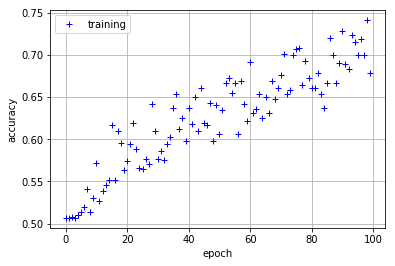
\includegraphics[scale=0.5]{p2q1a.png}
	
	As the epoch counter increases, the accuracy shows a increasing tendency.
	
	So if I increase the maximum number of epochs, the accuracy after the algorithm finishes will also increase. If I decrease the maximum number of epochs, the accuracy after the algorithm finishes will decrease.
	
	\item 
	The plot between epoch counter and the algorithm accuracy on both training and testing data:
	
	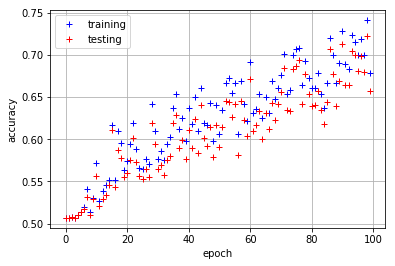
\includegraphics[scale=0.5]{p2q1b.png}
	
	Same as on the training data, as the epoch counter increases, the accuracy shows a increasing tendency on the testing data too.
	
	Compare to the plot on training data, the perceptron weights have lower accuracy on testing data. This indicates the algorithm overfits on the training data.
	
	\item 
	The accuracy of the perpeptron algorithm on the testing data after the last epoch is 0.6569563033651431.
	
	The confusion matrix is:
	
	\begin{tabular} {|c|c|c|}
		\hline
		 & Actual yes: $y = +1$ & Actual no: $y = -1$	\\ \hline
		Predicted yes: $\hat{y} = +1$& 299 & 0 \\ \hline
		Predicted no: $\hat{y} = -1$ & 683 & 1009 \\ \hline
	\end{tabular}

	\item 
	The ROC curves on training data with $w'$ and $w*$ are:
	
	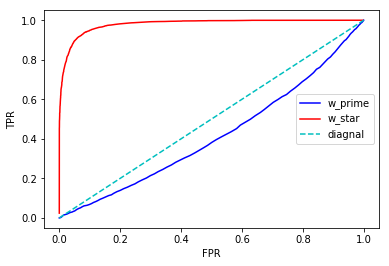
\includegraphics[scale=0.5]{p2q1d.png}
	
	The ROC curve depicts the trade off relationship between FPR and TPR, i.e., for a given FPR, what's the value of TPR. For a given FPR, we would prefer a higher TPR. So based on the comparison of ROCs, the weight vector $w*$ stands for a better decision boundary than $w'$.
	
	\item
	AUC for $w*$ is 0.9771385482873396.
	 
	AUC for $w'$ is 0.41607377087184255.
	
	AUC is the area under the ROC between $FPR = 0$ and $FPR = 1$. So if ROC reaches higher values more quickly, its corresponding AUC is larger. The approximated AUCs for two curves are consistent with their different shapes. AUC for $w*$ is approximately twice that of $w'$, meaning $w*$ leads to a better decision boundary.
	 
\end{enumerate}

\item 
\begin{enumerate}
	\item 
	The plot between epoch counter and the algorithm accuracy on training data is:
	
	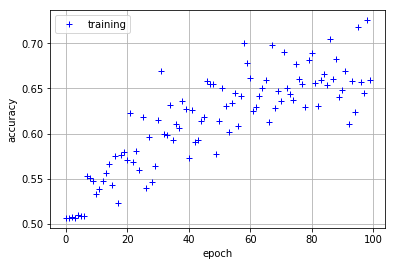
\includegraphics[scale=0.5]{p2q2a.png}
	
	The accuracy of the balanced winnow algorithm on the testing data is 0.6373681567051732.
	
	The confusion matrix on the testing data is:
	
	\begin{tabular} {|c|c|c|}
		\hline
		& Actual yes: $y = +1$ & Actual no: $y = -1$	\\ \hline
		Predicted yes: $\hat{y} = +1$& 260 & 0 \\ \hline
		Predicted no: $\hat{y} = -1$ & 722 & 1009 \\ \hline
	\end{tabular}

	\item 
	In question 2(a) I set $\eta = 0.1$. Now I try out $\eta = [0.2, 0.3, 0.4, 0.5]$, and compute the relationship between epoch counter and algorithm accuracy for each $\eta$. From the following plot, I find out that among the five values, $\eta = 0.1$ (the blue line) has the best performance in terms of algorithm accuracy.
	
	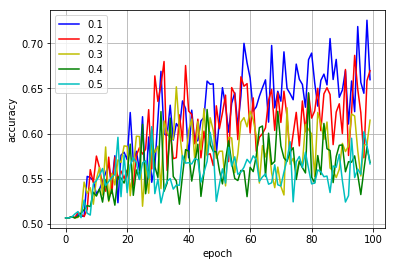
\includegraphics[scale=0.5]{p2q2b1.png}
	
	After this, I try $\eta = [0.02, 0.04, 0.06, 0.08]$ to see if smaller values would lead to even better accuracy. From the following plot, I think the performances of $\eta = [0.02, 0.04, 0.06, 0.08, 0.1]$ are similar to each other.
	
	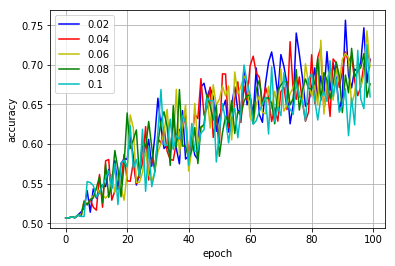
\includegraphics[scale=0.5]{p2q2b2.png}
	
	In general, to tune a parameter in an algorithm, I would try to use as many values of the parameter as possible, calculate certain reasonable measuring metrics of the algorithm under each parameter value, and see if some parameter values can lead to better performance of these measuring metrics.
\end{enumerate}
\end{enumerate}

\end{document}
